

\section{Sorting \XY}
\label{tree:related:xy}

\begin{figure}
	\centering
	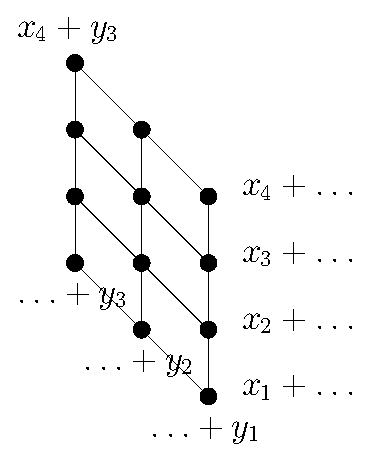
\includegraphics[height=0.2\textheight]{fig/related/x+y}
	\caption{Typical Hasse diagram for the Sorting \XY problem.}
	\label{fig:related:xy}
\end{figure}

We are given the following problem,

\begin{problem}
Given two sets of numbers \(X\) and \(Y\) each of cardinality \(n\), we want to
sort the set
\begin{displaymath}
X + Y = \enum{x + y \st x \in X, y \in Y}
\end{displaymath}
\end{problem}

The earliest known reference is \citet*{fredman:1976}, who attributes
the problem to Elwyn Berlekamp. As we can see in \ref{fig:related:xy}, this
problem fits in the \concept{SUPI} framework. However, we show later that
there are better ways to look at the structure of \XY.

Several geometric problems are known to be ``Sorting-(\XY)-hard'' (see
\citet*{barrera1996finding,barequet2001polygon}). Specifically, there
is a subquadratic-time transformation from sorting \XY to each of the
following problems: computing the Minkowski sum of two orthogonal-convex
polygons, determining whether one monotone polygon can be translated to fit
inside another, determining whether one convex polygon can be rotated to fit
inside another, sorting the vertices of a line arrangement, or sorting the
interpoint distances between $n$ points in $\R^d$.

\citet*{fredman:1976} also mentions an immediate application to multiplying
sparse polynomials. Let us explain. When we multiply polynomials, each of the
operands can be decomposed in terms. If polynomials $p$ and $q$ are of size $n$
and $m$, then the resulting polynomial contains $nm$ terms and the degree of
each term in the resulting polynomial is the sum of the degree of the operands
terms. Since sparse polynomials are usually stored in sorted order with respect
to the degree of their terms, we can easily see how the two problems are
related.

Concerning sorting \XY, the question of an optimal $\BigO{n^2}$ algorithm still
remains. Some additional references are \citet*{
harper:1975,
kahn:1995,
dietzfelbinger1989lower,
steiger1995pseudo,
lambert:1990,
erickson:1999,
bremner2012necklaces,
orourke:2012:sortxy}.
